\section{Details about Human Data Collection}


\paragraph{Mapping original reported statistics into the unified metric.}

\textbf{(Li; Breitmoser--Schweighofer-Kodritsch) AC/AC-B/2P under APV.}
These papers report Mean Absolute Deviation (MAD)\footnote{For clock auctions, since the winner did not submit a final sealed bid, the reported MAD is computed only from bidders who revealed a bid by dropping out (i.e., those who exited the clock), excluding the winner's unobserved terminal willingness-to-pay.}
 from truthful bidding. In Li (2017), the reported deviation is based on a group-level statistic involving the second-highest bid and second-highest value; in Breitmoser--Schweighofer-Kodritsch, deviations are computed from submitted bids (often focusing on non-winning bids). In each case we adhere to the paper's unit of observation, but the SMAD definition conceptually applies to the underlying submitted bids.
Because the equilibrium optimum under AC and 2P is truthful bidding $b^\star(v)=v$, we have $d_m=|b-v|$ and thus
\[
\Delta_m = 100\cdot \frac{\mathrm{MAD}_m}{\mu_m^\star},
\qquad
\mu_m^\star=\mathbb E[v].
\]
Here $\mathbb E[v]$ is implied by the experimental value distribution reported by the paper (e.g., $\mathbb E[v]=70$ in Li; and $\mathbb E[v]=65$ in Breitmoser--Schweighofer-Kodritsch given their stated common-value and idiosyncratic components).\footnote{When auctions are repeated, we follow the paper's convention and report post-learning blocks (e.g., dropping the first three rounds and using the next reported block).}
If the paper reports $\mathrm{SE}(\mathrm{MAD}_m)$ (often using group means as the unit of observation), we propagate it via
\[
\mathrm{SE}(\widehat{\Delta}_m)=100\cdot \frac{\mathrm{SE}(\widehat{\mathrm{MAD}}_m)}{\widehat{\mu}_m^\star},
\quad
\mathrm{CI}_{95\%}(\Delta_m)=\widehat{\Delta}_m \pm 1.96\,\mathrm{SE}(\widehat{\Delta}_m).
\]

\textbf{(Kagel--Levin 1993) First-/Second-/Third-price IPV.}
Kagel--Levin report bid regressions and over-/under-bidding frequencies for fixed bidder counts (e.g., $N\in\{5,10\}$). We treat each $N$ separately: the regression form $\hat b(x)=\hat\alpha+\hat\beta x$ is fit for a \emph{fixed} number of bidders, and is not pooled across varying $N$.
Theory gives linear equilibrium bid functions under IPV with $x\sim U[x_{\min},x_{\max}]$:

$$\begin{aligned}
b^\star_{\mathrm{FP\_IPV}}(x) &= x - \frac{x-x_{\min}}{N} = \frac{N-1}{N}x + \frac{1}{N}x_{\min} \\
b^\star_{\mathrm{SP\_IPV}}(x) &= x \\
b^\star_{\mathrm{TP\_IPV}}(x) &= x + \frac{x-x_{\min}}{N-2} = \frac{N-1}{N-2}x - \frac{1}{N-2}x_{\min}
\end{aligned}$$

(When $x_{\min}=0$, these reduce to the familiar slope-only formulas.)
Because only summary moments are reported, we reconstruct the bid distribution via a parametric data-generating process (DGP) consistent with Table~2.
For each auction series and fixed $N$, we assume $x\sim U[x_{\min},x_{\max}]$ (bounds from the paper), and generate bids as
\[
b = \hat\alpha+\hat\beta x + \varepsilon,\qquad \varepsilon\sim \mathcal N(\mu,\sigma^2),
\]
where $(\mu,\sigma)$ are calibrated by moment matching to the reported frequencies (e.g., $\Pr(b>x)$ and $\Pr(b>b^\star(x))$).
Given the calibrated DGP, we estimate
\[
\widehat{\mathrm{MAD}}_m = \mathbb E\!\left[\,|b-b^\star(x)|\,\right],
\qquad
\widehat{\mu}_m^\star=\mathbb E[b^\star(x)],
\qquad
\widehat{\Delta}_m = 100\cdot \frac{\widehat{\mathrm{MAD}}_m}{\widehat{\mu}_m^\star}.
\]
In practice, we run the Monte Carlo procedure 100 times and report the across-run mean $\widehat{\Delta}_m$ as the point estimate; uncertainty is obtained from across-run variability (percentile or normal approximation).


\textbf{(Levin--Kagel--Richard 1996 and related CV papers) First-price CV and English (second-price proxy).}
In common-value auctions, bidders observe signals $s_i$ about a common value $V$ (e.g., $s_i=V+\varepsilon_i$ as specified in the original paper). 

Theory gives linear equilibrium bid functions under Common Value:
$$\begin{aligned}
b^*_{FP\_CV}(x) &= x - \epsilon + Y\\
Y &= \left( \frac{2\epsilon}{N+1} \right) \exp\left[ -\left( \frac{N}{2\epsilon} \right) (x - (\underline{x} + \epsilon)) \right]\\
b^*_{SP\_CV}(x) &= x
\end{aligned}$$

The theoretical benchmark is the equilibrium bidding strategy $b_m^\star(s)$ implied by the paper's signal structure and mechanism. We therefore compute SMAD \emph{on bids} exactly as in private values:
\[
d_m = |b - b_m^\star(s)|,
\qquad
\Delta_m = 100\cdot \frac{\mathbb E[|b-b_m^\star(s)|]}{\widehat{\mu}_m^\star}.
\]

Because there is a very large common part in each players' valuation, we take the following normalization factor:
\[
{\widehat{\mu}_m^\star} = \mathbb E[b^\star_{max}(x) - b^\star_{min}(x)]
\]

When micro-data are unavailable, we reconstruct the bid distribution by simulating the paper's DGP (signals and value draws) together with the theoretical bidding rule $b_m^\star(\cdot)$, and calibrate any auxiliary noise parameters by moment matching to the summary statistics reported (e.g., frequencies of overbidding/high bids, or mean prices/profits as available). We run Monte Carlo 100 times and report the across-run mean $\widehat{\Delta}_m$ as the point estimate; uncertainty is obtained from across-run variability (percentile or normal approximation).

\subsection{Mixture Model Calibration Details}\label{app:mixture}

\begin{table}[h]
\centering
\small
\begin{tabular}{llcccc}
\toprule
Source & Treatment & $p_{\text{eq}}$ & $p_{\text{over}}$ & $\lambda$ & Calibration Target \\
\midrule
Li (2017) & 2P & 0.50 & 0.40 & 0.219 & Mean ratio = 1.08 \\
Li (2017) & AC & 0.67 & 0.18 & 0.198 & Mean ratio = 1.02 \\
Breitmoser (2022) & 2P & 0.44 & 0.40 & 0.283 & Mean ratio = 1.10 \\
Breitmoser (2022) & AC & 0.83 & 0.12 & 0.154 & Mean ratio = 1.01 \\
Kagel-Levin (1993) & FPSB, $n$=5 & 0.75 & 0.12 & 0.100 & $R^2$=0.88 \\
Kagel-Levin (1993) & SPSB, $n$=5 & 0.27 & 0.67 & 0.153 & $R^2$=0.97 \\
Kagel-Levin (1993) & TPSB, $n$=5 & 0.58 & 0.27 & 0.924 & $R^2$=0.94 \\
Gonczarowski (2022) & Traditional & 0.37 & 0.41 & 0.450 & MAD = \$0.51 \\
Gonczarowski (2022) & Menu & 0.34 & 0.43 & 0.450 & MAD = \$0.55 \\
\bottomrule
\end{tabular}
\caption{Calibrated mixture model parameters by source and treatment. Mixture weights from reported rates; $\lambda$ calibrated to match secondary statistic listed; $p_{\text{under}} = 1 - p_{\text{eq}} -
p_{\text{over}}$.}
\label{tab:calibration}
\end{table}

\section{LLM Simulation Procedure}

We give the prompt-and-parse pipeline used to simulate various auctions with LLM agents. Each simulated bidder is queried independently. In every auction instance, the agent (i) receives the scenario and mechanism description, (ii) is asked to articulate a short bidding plan, and (iii) outputs a bid/decision in a structured format that can be parsed deterministically.


\subsection{Simulation process in sealed-bid auctions}\label{app:process}

\paragraph{Prompt structure.}
We attach the canonical prompt template in the following. Each bidder is assigned a role (e.g., ``Bidder Andy'') and informed of the other bidders' identities. The prompt then provides (a) a mechanism-specific \emph{rule explanation} (e.g., first-price vs.\ second-price vs.\ third-price), and (b) universal \emph{instructions} that define the objective and response format. We require the model to respond using two exact tags: \verb|<PLAN>| (a brief natural-language rationale) and \verb|<ACTION>| (the bid as a number) in the Chain-of-Thought style \citet{wei2022chain}:


\begin{figure}[H]
\centering
\begin{minipage}{0.95\textwidth}
\begin{lstlisting}
    You are Bidder Andy.            
    You are bidding with {OTHER_BIDDERS}.     
    
    {RULE EXPLANATION} + {INSTRUCTIONS}

    Your response must use these EXACT tags below:
    ```
    <PLAN>[ Reason out a bidding strategy and plan for this round. {% if current_round > 1 %}Learn from your previous rounds. Remember: the values will be different in future rounds - don't assume patterns will repeat. {% else %}Consider the history above if available. {% endif %}Be detailed and precise. LIMIT your plan to 100 words. ] </PLAN>
    <ACTION> [Your bid amount as a number, e.g., 1, 44, 50] </ACTION>
    ```
\end{lstlisting}
\end{minipage}
\end{figure}


\paragraph{Universal objective instruction.}
Across all sealed-bid simulations, we append a universal instruction block that specifies the optimization objective (maximize profit) and discourages spurious cross-round pattern extrapolation \citet{fish2024algorithmic}. We report the exact text in the following.
\begin{figure}[H]
\centering
\begin{minipage}{0.95\textwidth}
\begin{lstlisting}
    Your TOP PRIORITY is to place bids which maximize the user's profit in the long run. 
    Learn from the history of previous rounds in order to maximize your total profit. 
    Don't forget the values are redrawn independently each round.
\end{lstlisting}
\end{minipage}
\end{figure}

\paragraph{History and feedback (multi-round ablation only).}
Our main experiments restrict attention to single-round auctions ($T=1$). When we run the multi-round ablation in Appendix~\ref{app:learning}, we include a standardized history transcript in the prompt. The history contains the agent's past realized values, past bids, whether it won, the transaction price, and realized profit, as well as the list of all bids in each prior round. This transcript is appended above the response-tag requirements, so that the agent can condition on past outcomes without ambiguity.




\subsection{Simulation process in Ascending Clock auctions}\label{app:dynamic}

In Ascending Clock Auctions, each round consists of multiple clock cycles, during which every bidder is asked whether they want to stay or drop out at the current clock price.
In the first round, bidders are reminded of the auction rules, similar to those outlined in Section \ref{app:process}. 
The auction starts with an initial price of 0, which increases incrementally until only one bidder remains or two bidders drop out simultaneously, in which case the winner is chosen randomly. 
The detailed prompt is listed as follows, with variables enclosed in brackets:

\begin{figure}[H]
\centering
\begin{minipage}{0.95\textwidth}
\begin{lstlisting}
    You are Bidder Andy. You are bidding with {OTHER_BIDDERS}.     
    
    {RULE EXPLANATION} + {INSTRUCTIONS} 

    Your value towards to the prize is 26 in this round.
    The current price in this clock cycle is {current_price}. 
    The price for next clock cycle is {current_price + increment}.

    The previous bidding history is: {transcript}.

    Do you want to stay in the bidding? 
    If you choose yes, you can keep bidding for next clock. If you choose No, you will exit and have no chance to re-enter the bidding. Your response must use these EXACT tags below. You must output the ACTION.
    ```
    <PLAN>
    [Write your plans for bidding strategies. Be detailed and precise but keep things succinct and don't repeat yourself. LIMIT your plan to 50 words. ] </PLAN>
    <ACTION> Yes or No </ACTION>
    ```
\end{lstlisting}
\end{minipage}
\label{fig:ac_prompt}
\end{figure}

In AC, if LLM bidders didn't decide to drop out in the first round, they are shown the previous bidding history for the next clock cycle. The history includes the price and how many people had dropped out. 
And the transcript variable will be the following format:
\textit{    The previous biddings are: 
    ['In clock round 1, the price was 1, 
    no players dropped out'].}

In AC-B, we don't show the previous biddings and in each clock cycle, we directly query LLM agents' decision. 
So the transcript variable will be None.

A clock auction round ends when only one bidder remains, who is declared the winner, or when two bidders drop out simultaneously, in which case the winner is chosen randomly. Each auction consists of 10 independent rounds with affiliated value settings.



\subsection{Simulation process in eBay auctions}\label{app:ebay}

For eBay auctions, we discretize the continuous bidding period into 10 periods. Each period, LLM agents decide whether to increase their bid or hold their current bid. The bidding process follows a structured format, where bidders act in a predefined sequence each period (e.g., Charles, then Alice, then Betty). Agents are informed of past price changes through a transcript, such as ``On day 1, the price changed to 1. On day 2, the price changed to 3.''

The prompt provides key details, including the bidder's private value, the total number of bidding days, the current day, the bidding order, previous bids, previous proxy bids, and the current price. The decision-making process is again guided by a structured asking prompt that enforces bidding rules. 
\begin{figure}[H]
\centering
\begin{minipage}{0.95\textwidth}
\begin{lstlisting}
    You are Bidder Andy.            
    You are bidding with {OTHER_BIDDERS}.     
    
    {RULE EXPLANATION} + {INSTRUCTIONS} 
    
    Your private value for this item is ${private_value}. This is the maximum amount you are willing to pay. Keep this value private. There are in total {total_periods} days  of bidding and this is day {current_period}. {ordering}.
    
    Your previous bids are {previous_bid}. If you have already placed bids, you can only increase your bid or hold your current bid. The previous proxy bids are: {transcript}.
    The current price is {current_price}.
    Your response must use these EXACT tags below. Don't miss the amount.
    ```
    <PLAN>[Write your plans for what bidding strategies to test next. Be detailed and precise but keep things succinct and don't repeat yourself. LIMIT your plan to 50 words. ]</PLAN>
    <CHECK>your last bid is {{last_bid_amount}}, you cannot bid lower that this value </CHECK>
    <ACTION> BID or HOLD  </ACTION>
    <AMOUNT> if BID, enter a number here, e.g. 1, 44. If HOLD, enter 0 </AMOUNT>
    ```
\end{lstlisting}
\end{minipage}
\label{fig:ebay_prompt}
\end{figure}



\section{Examining Learning Effects in Repeated Games}\label{app:learning}

To assess whether LLM agents exhibited learning or adaptation across rounds, we conduct a set of statisitcal tests comparing early-round behavior to late-round behavior and examining continuous trends over time. For the First-Price Sealed-Bid (FPSB) auction, the mean SMAD in the first five rounds (0.2523) is essentially identical to that in the last five rounds (0.2524), with no detectable difference in either a t-test ($p = 0.9968$) or a Mann–Whitney U test ($p = 0.9131$). Trend analyses likewise show no evidence of systematic change: a linear regression yields a slope indistinguishable from zero (p = 0.9886) and a Spearman test finds no monotonic movement ($\rho = 0.0929$, $p = 0.7420$). Results are similar for the Second-Price Sealed-Bid (SPSB) auction. The comparison between the first and last five rounds reveals no significant difference (means 0.1282 vs. 0.1447; t-test $p = 0.3335$; Mann–Whitney $p = 0.1948$), and neither a linear trend test (p = 0.3664) nor a Spearman correlation test ($\rho= 0.3964$, $p = 0.1435$) indicates meaningful temporal structure. Taken together, across all specifications, we find no statistical evidence of learning effects, behavioral drift, or systematic changes in bidding deviations over the 15 rounds. LLM agents' deviation magnitudes remain remarkably stable throughout both FPSB and SPSB environments.

\begin{figure}[H]
    \centering
    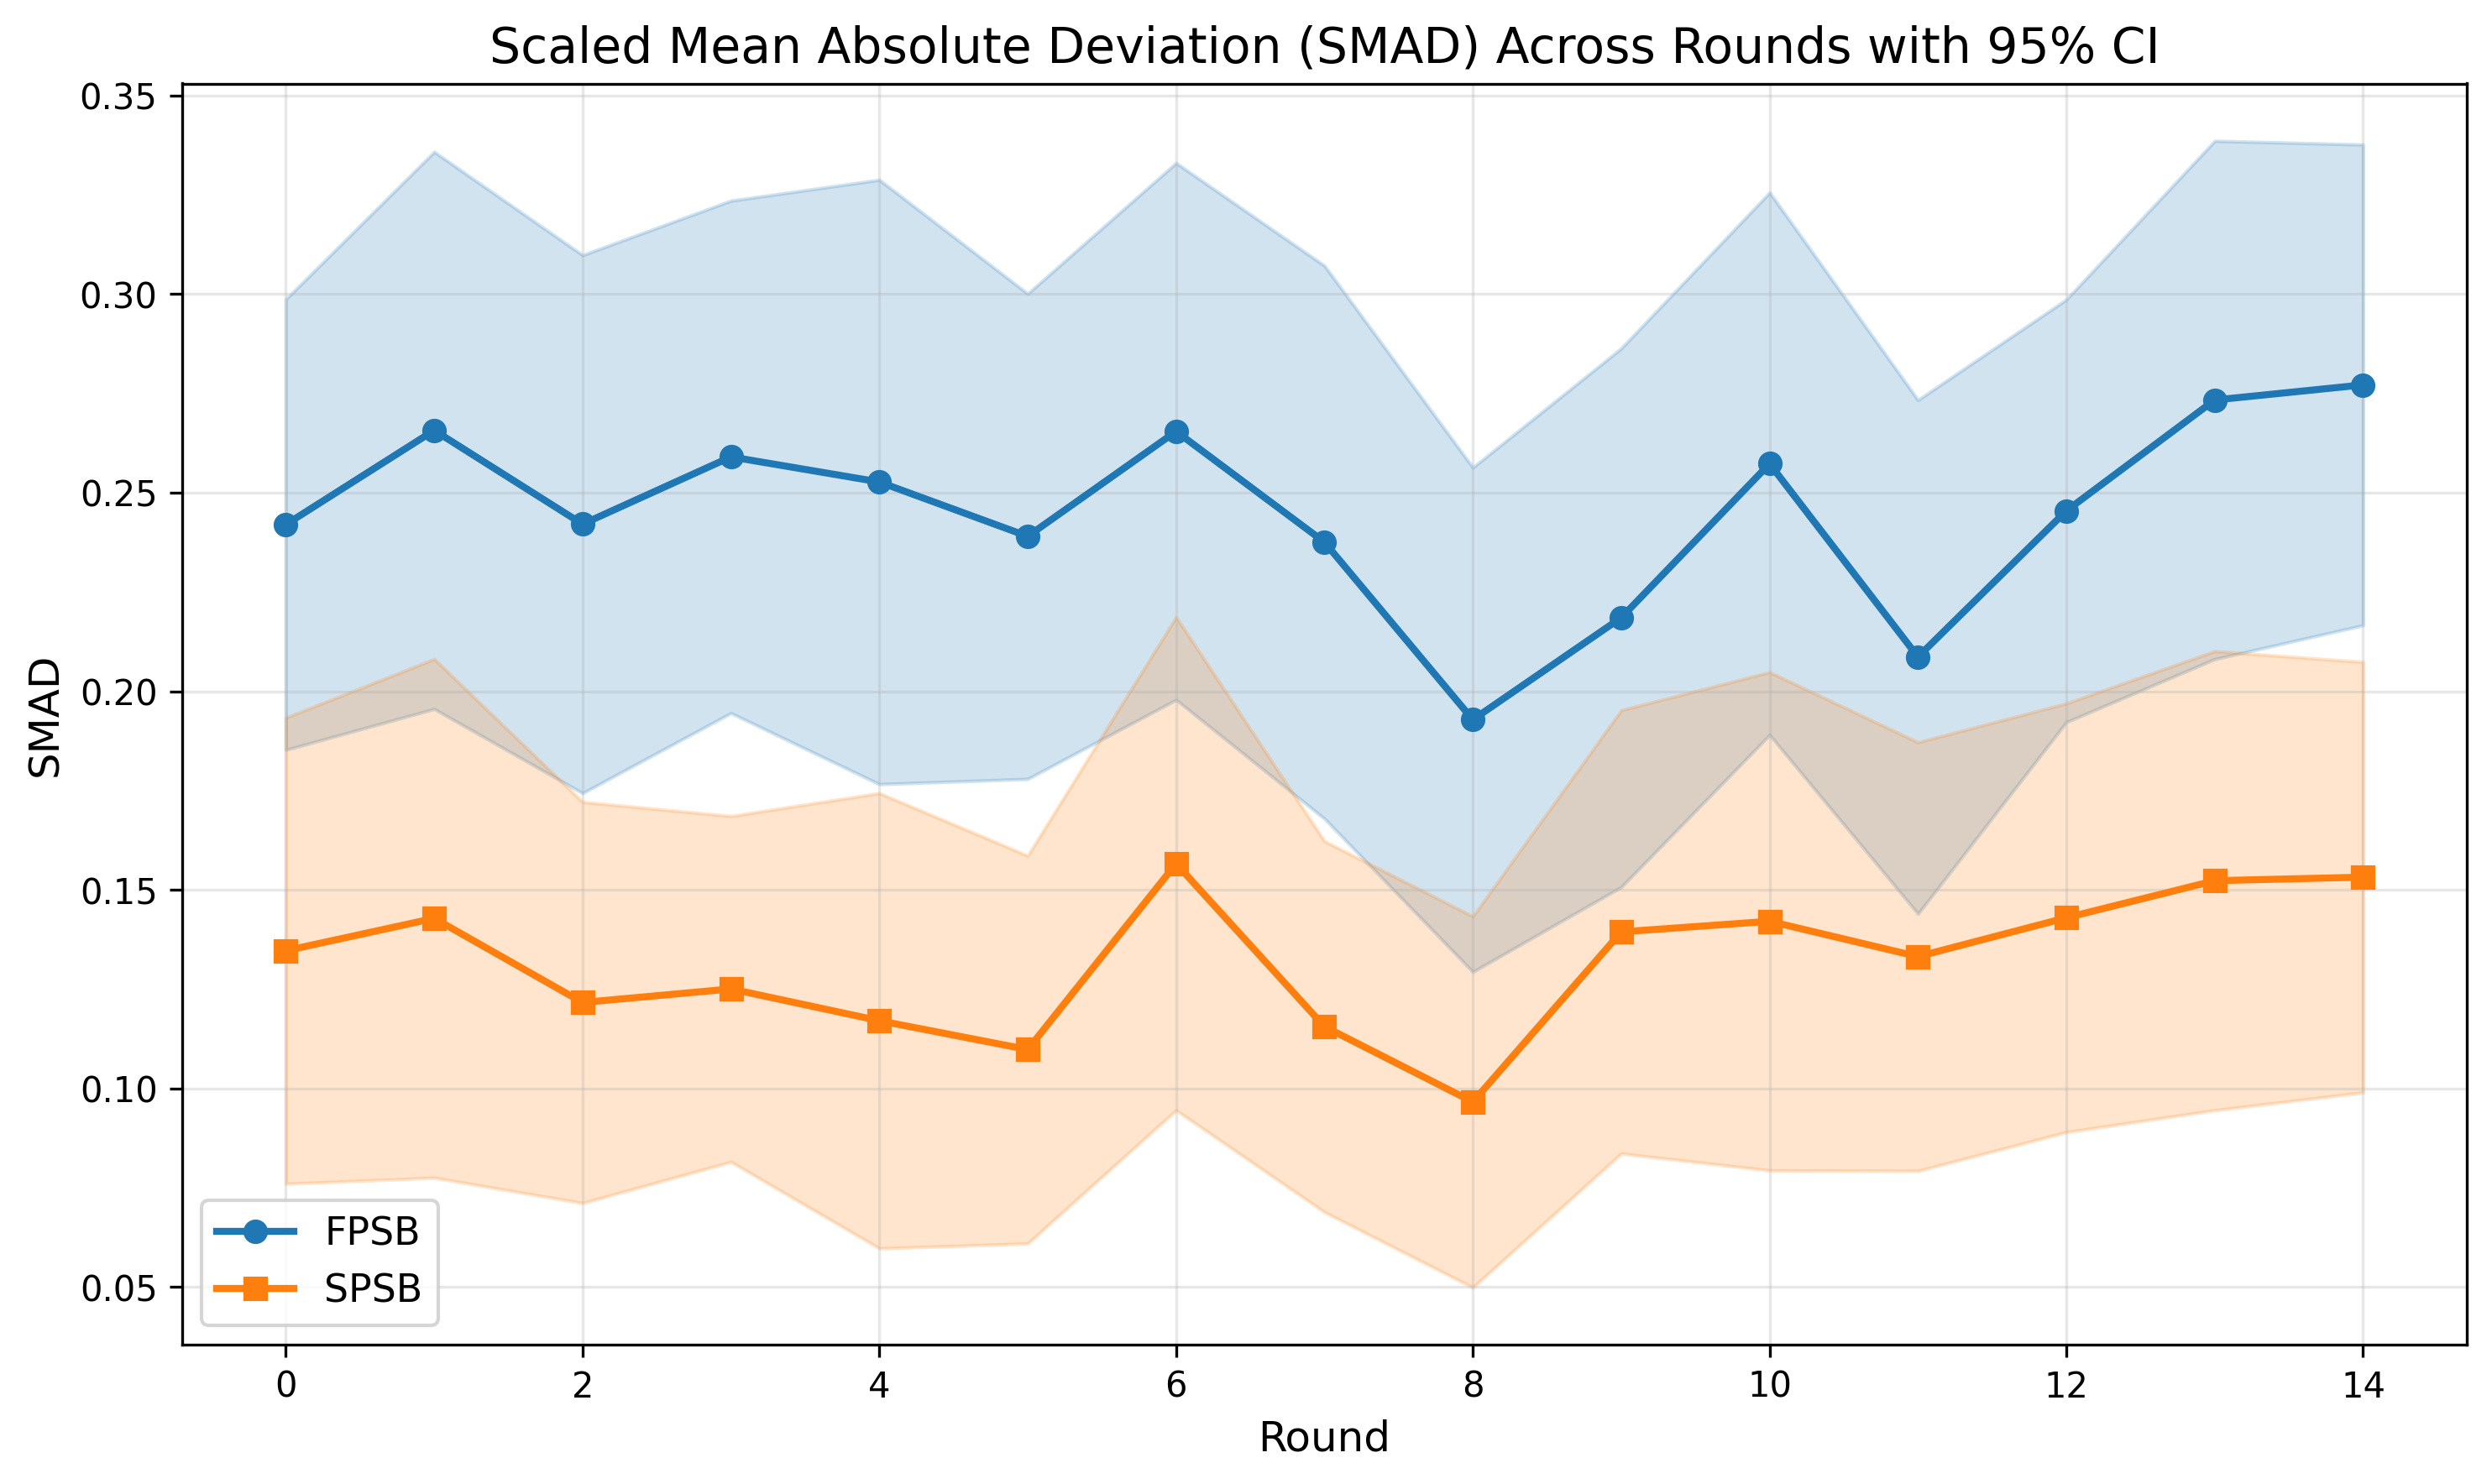
\includegraphics[scale=0.45]{figures/smad_rounds.png}
    \caption{ Multiple-round simulation of First-Price and Second-Price sealed-bid auction with GPT-4o model (Temp=0.5). Y-axis stands for Scaled Mean Absolute Deviation (SMAD) between actual bidding and optimal bidding.
    \label{fig:multiple-round}}
\end{figure}

\section{Ablation on Models and Parameters}
\subsection{Varying Temperature for GPT-4o Agent}
We examined the effect of the temperature parameter (T $\in$ \{0.1, 0.5, 1.0\}) on GPT-4o's 
bidding behavior across seven auction formats. The temperature parameter controls the 
randomness of the model's outputs, with lower values producing more deterministic 
responses and higher values introducing more variability.


The overall impact of temperature on bidding performance is relatively modest
across auction types.
The reduced variation at T=0.1 produces
more consistent outputs but appears to limit the model's ability to approximate optimal
strategies, particularly in auction formats requiring nuanced strategic reasoning. For
general-purpose auction applications, T=1.0 or T=0.5 provide better balance between
consistency and strategic flexibility, though format-specific tuning can yield marginal
improvements in performance.


\begin{figure}[H]
    \centering
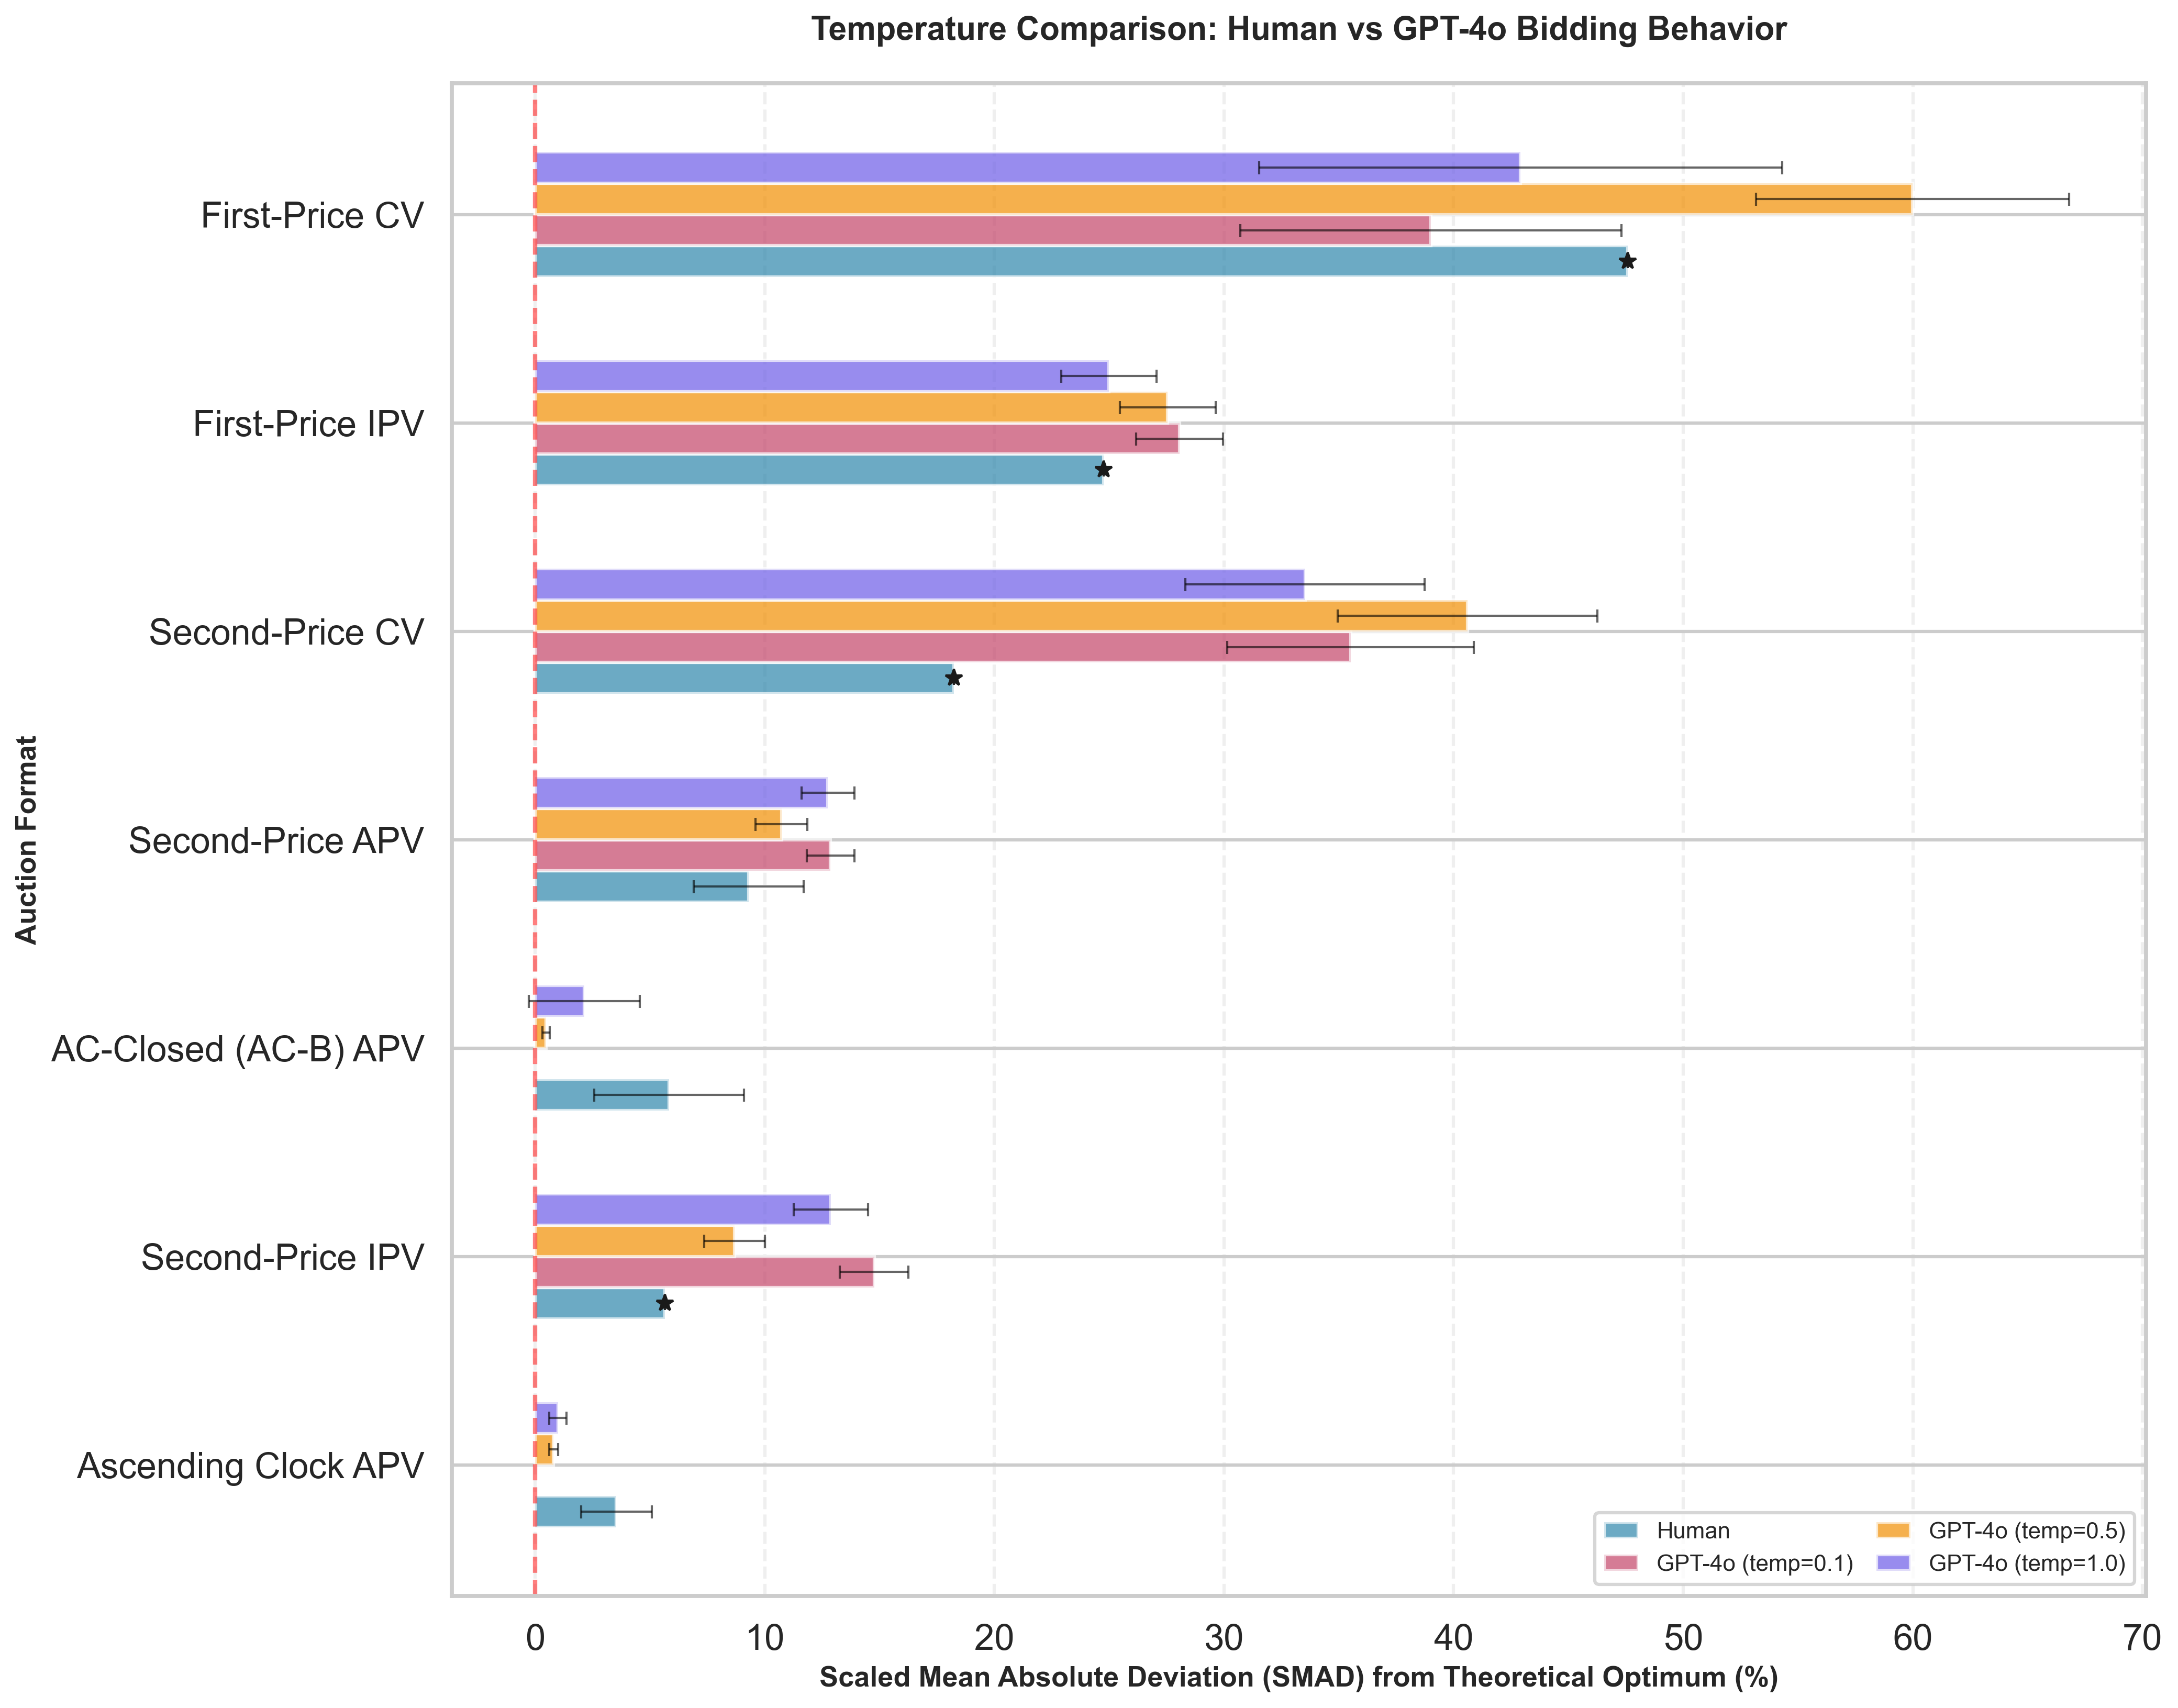
\includegraphics[scale=0.35]{figures/appendix2_temperature_comparison.png}
    \caption{Comparison of the bidding behavior of human participants and GPT-4o across three
different temperature settings (T=0.1, 0.5, 1.0) in seven auction formats. The horizontal
bars represent the Scaled Mean Absolute Deviation (SMAD) from theoretical equilibrium,
with error bars indicating 95\% confidence intervals.
    \label{fig:temperature}}
\end{figure}


\begin{table}[htbp]
\centering
\begin{tabular}{l|ccc}
\hline
Auction Format & $T=0.1$ & $T=0.5$ & $T=1.0$ \\
\hline
AC-Closed (AC-B) APV & 0.00 & 0.47 & 2.15 \\
Ascending Clock APV & 0.00 & 0.81 & 1.00 \\
Second-Price IPV & 14.77 & 8.69 & 12.89 \\
Second-Price APV & 12.87 & 10.73 & 12.75 \\
First-Price CV & 39.00 & 59.99 & 42.92 \\
Second-Price CV & 35.51 & 40.60 & 33.53 \\
First-Price IPV & 28.07 & 27.55 & 24.99 \\
\hline
\end{tabular}
\caption{Temperature Effects on Bidding Behavior (SMAD \%). Note: SMAD = Scaled Mean Absolute Deviation from theoretical equilibrium.}
\label{tab:temperature_comparison}
\end{table}



\subsection{Varying the Base Models for LLM bidding}

We compare the bidding behavior of four frequently used large language models against human participants
across seven auction formats. All LLMs are tested at temperature=0.5 to ensure fair
comparison. The models tested are: Claude Sonnet 3.5, Gemini-2.0 Flash, GPT-5-mini
(reasoning model), and Llama-3-8B-Instruct (open-sourced model).

GPT-5-mini, as a reasoning model, demonstrates remarkably low deviation from theoretical equilibrium (mean SMAD = 6.68\%), with near-perfect performance in ascending clock and first-price formats. In stark contrast, Llama exhibits substantially poor performance across all auction formats (mean SMAD = 57.58\%), significantly exceeding human baselines in 6 out of 7 formats, suggesting that raw model size alone is insufficient for complex strategic reasoning. 
Claude and Gemini show moderate performance, falling between these extremes.

\begin{figure}[H]
    \centering

\includegraphics[scale=0.375]{figures/appendix2_model_comparison.png}
    \caption{Comparison of the bidding behavior of human participants and LLM agents across four other foundation models (GPT-5-mini, Claude Sonnet 3.5, Gemini-2.0 Flash and Llama-3-8B-Instruct) in seven auction formats. The horizontal
bars represent the Scaled Mean Absolute Deviation (SMAD) from theoretical equilibrium,
with error bars indicating 95\% confidence intervals.
    \label{fig:model_ablation}}
\end{figure}


\begin{table}[htbp]
\centering
\begin{tabular}{l|c|cccc}
\hline
\multirow{2}{*}{Auction Format} & Human & Claude & Gemini & GPT-5 & Llama \\
 & SMAD & SMAD & SMAD & SMAD & SMAD \\
\hline
First-Price IPV & 24.76 & 24.09 & 27.05 & 0.08*** & 38.16*** \\
Second-Price IPV & 5.65 & 9.72*** & 3.01*** & 0.20*** & 54.89*** \\
AC-Closed (AC-B) APV & 5.83 & 0.00*** & 1.26*** & 0.00*** & 67.00* \\
Second-Price APV & 9.31 & 9.58 & 8.02 & 1.36*** & 53.08*** \\
Ascending Clock APV & 3.54 & 5.74* & 0.00*** & 0.00*** & 104.10*** \\
First-Price CV & 47.59 & 54.07 & 59.50 & 30.22*** & 53.68 \\
Second-Price CV & 18.23 & 27.19* & 30.89** & 14.80 & 32.27* \\
\hline
\end{tabular}
\caption{Model Comparison: Bidding Behavior across Auction Formats. Note: SMAD = Scaled Mean Absolute Deviation from theoretical equilibrium. 
All LLMs tested at temperature=0.5. 
Significance stars indicate difference from human baseline: * p<0.05, ** p<0.01, *** p<0.001. }
\label{tab:model_comparison}
\end{table}


 \section{Additional Analysis for eBay-Proxy Auctions}
 
 \begin{figure}[H]
    \centering 
\includegraphics[scale = .45]{figures/ebay_revenue_by_type.png}
    \caption{\textbf{eBay Revenue by Auction Type, IPV environment} No significant different between any of the settings. 
    \label{fig:ebay_revenue}}
\end{figure}

    \begin{table}
        \begin{tabular}{l l c c}
            \toprule
            Auction Type 1 & Auction Type 2 & t-statistic & p-value \\
            \midrule
            \texttt{basic\_proxy} & \texttt{closing\_rule} & \(0.020\) & \(0.984\) \\
            \texttt{basic\_proxy} & \texttt{hidden\_reserve\_40} & \(-0.026\) & \(0.98\) \\
            \texttt{basic\_proxy} & \texttt{hidden\_reserve\_50} & \(-0.096\) & \(0.923\) \\
            \texttt{basic\_proxy} & \texttt{hidden\_reserve\_60} & \(-0.071\) & \(0.944\) \\
            \texttt{basic\_proxy} & \texttt{closing\_rule\_hidden\_40} & \(-0.109\) & \(0.913\) \\
            \texttt{basic\_proxy} & \texttt{closing\_rule\_hidden\_50} & \(-0.109\) & \(0.913\) \\
            \texttt{basic\_proxy} & \texttt{closing\_rule\_hidden\_60} & \(-0.119\) & \(0.905\) \\
            \texttt{closing\_rule} & \texttt{hidden\_reserve\_40} & \(-0.047\) & \(0.963\) \\
            \texttt{closing\_rule} & \texttt{hidden\_reserve\_50} & \(-0.120\) & \(0.905\) \\
            \texttt{closing\_rule} & \texttt{hidden\_reserve\_60} & \(-0.093\) & \(0.926\) \\
            \texttt{closing\_rule} & \texttt{closing\_rule\_hidden\_40} & \(-0.133\) & \(0.895\) \\
            \texttt{closing\_rule} & \texttt{closing\_rule\_hidden\_50} & \(-0.133\) & \(0.895\) \\
            \texttt{closing\_rule} & \texttt{closing\_rule\_hidden\_60} & \(-0.144\) & \(0.886\) \\
            \texttt{hidden\_reserve\_40} & \texttt{hidden\_reserve\_50} & \(-0.071\) & \(0.944\) \\
            \texttt{hidden\_reserve\_40} & \texttt{hidden\_reserve\_60} & \(-0.045\) & \(0.964\) \\
            \texttt{hidden\_reserve\_40} & \texttt{closing\_rule\_hidden\_40} & \(-0.083\) & \(0.934\) \\
            \texttt{hidden\_reserve\_40} & \texttt{closing\_rule\_hidden\_50} & \(-0.083\) & \(0.934\) \\
            \texttt{hidden\_reserve\_40} & \texttt{closing\_rule\_hidden\_60} & \(-0.093\) & \(0.927\) \\
            \texttt{hidden\_reserve\_50} & \texttt{hidden\_reserve\_60} & \(0.026\) & \(0.98\) \\
            \texttt{hidden\_reserve\_50} & \texttt{closing\_rule\_hidden\_40} & \(-0.013\) & \(0.99\) \\
            \texttt{hidden\_reserve\_50} & \texttt{closing\_rule\_hidden\_50} & \(-0.013\) & \(0.99\) \\
            \texttt{hidden\_reserve\_50} & \texttt{closing\_rule\_hidden\_60} & \(-0.020\) & \(0.984\) \\
            \texttt{hidden\_reserve\_60} & \texttt{closing\_rule\_hidden\_40} & \(-0.038\) & \(0.97\) \\
            \texttt{hidden\_reserve\_60} & \texttt{closing\_rule\_hidden\_50} & \(-0.038\) & \(0.97\) \\
            \texttt{hidden\_reserve\_60} & \texttt{closing\_rule\_hidden\_60} & \(-0.046\) & \(0.963\) \\
            \texttt{closing\_rule\_hidden\_40} & \texttt{closing\_rule\_hidden\_50} & \(0.000\) & \(1\) \\
            \texttt{closing\_rule\_hidden\_40} & \texttt{closing\_rule\_hidden\_60} & \(-0.006\) & \(0.995\) \\
            \texttt{closing\_rule\_hidden\_50} & \texttt{closing\_rule\_hidden\_60} & \(-0.006\) & \(0.995\) \\
            \bottomrule
        \end{tabular}
            \caption{Pairwise t-tests for seller revenue differences across auction types. None of the comparisons show significant revenue differences.       \label{tab:revenue_tests}}
    \end{table}
% \end{figure}






\newpage

\section{Auction Rule Prompts}\label{app:prompt}
Below, we report the prompts used for each section.

\subsection{Independent Private Values Prompts}\label{sec:ipv-prompts}
Following the simulation procedure outlined in Section~\ref{app:process}, we employ the following prompts for the four auctions tested in this section. For each prompt, only the third paragraph (describing the allocation rule and payment) differ. For the FPSB, we describe the auction format as follows:
\begin{figure}
\centering
\begin{minipage}{0.95\textwidth}
\begin{lstlisting}
In this game, you will participate in an auction for a prize against {{num_bidders}} other bidders. You will play this game for {{n}} rounds.
At the start of each round, bidders will see their value for the prize, randomly drawn between $0 and ${{private}}, with all values equally likely.
After learning your value, you will submit a bid privately at the same time as the other bidders. Bids must be in ${{increment}} increments.
The highest bidder wins the prize and pays their bid amount. If you win, your earnings will increase by your value for the prize, and decrease by your bid. If you don't win, your earnings will remain unchanged.
After each auction, we will display all bids. Ties for the highest bid will be resolved randomly.
\end{lstlisting}
\end{minipage}
\label{fig:sealbid_prompt}
\end{figure}


For the SPSB, we describe the auction format as follows:
\begin{figure}
\centering
\begin{minipage}{0.95\textwidth}
\begin{lstlisting}
In this game, you will participate in an auction for a prize against {{num_bidders}} other bidders. You will play this game for {{n}} rounds.
At the start of each round, bidders will see their value for the prize, randomly drawn between $0 and ${{private}}, with all values equally likely.
After learning your value, you will submit a bid privately at the same time as the other bidders. Bids must be in ${{increment}} increments.
The highest bidder wins the prize and pays the second-highest bid. If you win, your earnings will increase by your value for the prize, and decrease by the second-highest bid. If you don't win, your earnings will remain unchanged.
After each auction, we will display all bids. Ties for the highest bid will be resolved randomly.
\end{lstlisting}
\end{minipage}
\label{fig:sealbid_prompt}
\end{figure}


For the TPSB, we describe the auction format as follows:
\begin{figure}
\centering
\begin{minipage}{0.95\textwidth}
\begin{lstlisting}
In this game, you will participate in an auction for a prize against {{num_bidders}} other bidders. You will play this game for {{n}} rounds.
At the start of each round, bidders will see their value for the prize, randomly drawn between $0 and ${{private}}, with all values equally likely.
After learning your value, you will submit a bid privately at the same time as the other bidders. Bids must be in ${{increment}} increments.
The highest bidder wins the prize and pays the third-highest bid. If you win, your earnings will increase by your value for the prize, and decrease by the third-highest bid. If you don't win, your earnings will remain unchanged. If there are less than three bids, no one will win the auction.
After each auction, we will display all bids. Ties for the highest bid will be resolved randomly.
\end{lstlisting}
\end{minipage}
\label{fig:sealbid_prompt}
\end{figure}


\subsection{Obviously Strategy-Proof Prompts}\label{sec:osp-prompts}
The sealed-bid prompt follows the style of the last section's prompts closely. The only difference is in the first two paragraphs, where agents are informed of the APV environment. For the SPSB, we describe the auction format as follows:
\begin{figure}
\centering
\begin{minipage}{0.95\textwidth}
\begin{lstlisting}
In this game, you will participate in an auction for a prize against {{num_bidders}} other bidders. You will play this game for {{n}} rounds.
At the start of each round, bidders will see their value for the prize. Your value for the prize will be calculated as follows:
1. First we will randomly draw a common value between {{common_low}} and {{common_high}}, with all values equally likely.
2. Then, for each bidder, a private taste adjustment will be drawn between 0 and {{private}}, with all values equally likely.
Your value for the prize is equal to the common value plus your private taste adjustment. You will not learn the common value or your private taste adjustment separately. This means that each person in your group may have a different value for the prize. However, if you have a high value, it is more likely that other people in your group have a high value.
After learning your value, you will submit a bid privately at the same time as the other bidders. Bids must be in ${{increment}} increments. 
The highest bidder wins the prize and pays the second-highest bid. If you win, your earnings will increase by your value for the prize, and decrease by the second-highest bid. If you don't win, your earnings will remain unchanged.
After each auction, we will display all bids. Ties for the highest bid will be resolved randomly.
\end{lstlisting}
\end{minipage}
\label{fig:sealbid_prompt}
\end{figure}

The implementation of the clock auction simulates a global clock price, with prices beginning at $0$ and increasing in $\$1$ increments. The clock auction format descriptions closely mirror the SPSB format above, but with the added description of the clock mechanism in the fourth and fifth paragraphs. 
In the AC auction, we describe the auction format as follows: 
\begin{figure}
\centering
\begin{minipage}{0.95\textwidth}
\begin{lstlisting}
In this game, you will participate in an auction for a prize against {{num_bidders}} other bidders. You will play this game for {{n}} rounds. 
At the start of each round, bidders will see their value for the prize. Your value for the prize will be calculated as follows:
1. First we will randomly draw a common value between {{common_low}} and {{common_high}}, with all values equally likely.
2. Then, for each bidder, a private taste adjustment will be drawn between 0 and {{private}}, with all values equally likely.
Your value for the prize is equal to the common value plus your private taste adjustment. You will not learn the common value or your private taste adjustment separately. This means that each person in your group may have a different value for the prize. However, if you have a high value, it is more likely that other people in your group have a high value.
The auction proceeds as follows: First, you will learn your value for the prize. Then, the auction will start. We will display a price to everyone in your group that starts at 0 and counts upwards in {{increment}} USD increments, up to a maximum of {{common_high + private}}. At any point, you can choose to leave the auction, and anytime a bidder leaves, we will broadcast that information to all the remaining bidders. 
When there is only one bidder left in the auction, that bidder will win the prize at the current price. If you win, your earnings will increase by your value for the prize, and decrease by the current price. If you don't win, your earnings will remain unchanged.
After each auction, we will display all bids. Ties for the highest bid will be resolved randomly.
\end{lstlisting}
\end{minipage}
\label{fig:sealbid_prompt}
\end{figure}

The AC-B auction description closely resembles the AC format, but with the explicit caveat that we will not notify bidders when competitors drop out.


\subsection{Common Value Auctions}

For the Second-Price Sealed-Bid auction in the Common Value setting, the rule is

\begin{figure}[H]
\centering
\begin{minipage}{0.95\textwidth}
\begin{lstlisting}
In this game, you will participate in an auction for a prize against {{num_bidders}} other bidders. You will play this game for {{n}} rounds. 
At the start of each round, bidders will see their perceived value for the prize- a noisy measurement of the true value of the prize. Your perceived value for the prize will be calculated as follows:
1. For each round, a common value will be drawn between {{common_low}} and {{common_high}}, with all values equally likely to be drawn.
2. For each person, a private noisy adjustment will be drawn between -{{private}} and {{private}}, with all values equally likely to be drawn.
We will tell you your perceived value, the sum of the common value and the private noise adjustment. However, everyone's true value for the prize is equal to the shared common value. 
After learning your perceived value, you will submit a bid privately at the same time as the other bidders. Bids must be in ${{increment}} increments. 
The highest bidder wins the prize and pays the second-highest bid. If you win, your earnings will increase by the true value for the prize, and decrease by the second-highest bid. If you don't win, your earnings will remain unchanged.
After each auction, we will display all bids. Ties for the highest bid will be resolved randomly.
\end{lstlisting}
\end{minipage}
\label{fig:sealbid_prompt}
\end{figure}


\subsection{Ebay-proxy prompt}
For the Standard eBay auction with proxy bidding (T1), the rule is:
\begin{figure}[H]
\centering
\begin{minipage}{0.95\textwidth}
\begin{lstlisting}
In this game, you will participate in an eBay auction for an item against {{num_bidders}} other bidders. This auction will last for {{num_rounds}} days. All dollar amounts in this game are in US Dollars ($).

Item Details:
Item Description: {{item_description}}
Item Condition: {{item_condition}}
Your Private Value: At the start of each round, bidders will see their value for the item, randomly drawn between $0 and ${{private}}, with all values equally likely. After learning your value for the item, you will submit a maximum bid. Bids must be in ${{increment}} increments.

Auction Format:
This is an eBay auction. The auction starts at ${{start_price}} and will last for {{num_rounds}} days. eBay uses "proxy bidding." This means that if you wish to enter the auction, you should submit your maximum bid, and eBay will automatically bid on your behalf, up to your maximum, only as much as necessary to maintain your position as the highest bidder. Each day you will see the current price and have the opportunity to increase your maximum bid. If you do not want to increase your maximum bid, then output HOLD.

You may place bids at any point during the auction, even on the final day. No bidder will know if they (or anyone else) is the last bidder on the final day.

The highest bidder wins the prize and pays the auction price at the time the auction's clock expired. If you win, your earnings will increase by your value for the prize, and decrease by the final auction price. If you don't win, your earnings will remain unchanged. Ties for the highest bid will be resolved randomly.
\end{lstlisting}
\end{minipage}
\label{fig:sealbid_prompt}
\end{figure}


For the eBay auction with a modified closing rule (T2), the updated closing rule in the prompt is

\begin{figure}[H]
\centering
\begin{minipage}{0.95\textwidth}
\begin{lstlisting}
This auction also has a closing rule. This means that if a new maximum bid is placed on the last day, the auction will automatically extend by another day. This extension will continue to be applied as long as new maximum bids are placed on the final day. No bidder will know if they (or anyone else) is the final bidder on the last day.
\end{lstlisting}
\end{minipage}
\label{fig:sealbid_prompt}
\end{figure}


For the standard eBay auction with a hidden reserve price (T3), the item detail prompt is the same but the rule is changed to:
\begin{figure}[H]
\centering
\begin{minipage}{0.95\textwidth}
\begin{lstlisting}
Auction Format:
This is an eBay auction with a hidden reserve price. The auction starts at ${{start_price}} and will last for {{num_rounds}} days. eBay uses "proxy bidding." This means that if you wish to enter the auction, you should submit your maximum bid, and eBay will automatically bid on your behalf, up to your maximum, only as much as necessary to maintain your position as the highest bidder. Each day you will see the current price and have the opportunity to increase your maximum bid. If you do not want to increase your maximum bid, then output HOLD.

You may place bids at any point during the auction, even on the final day. However, if no bidder produces a maximum bid above the hidden reserve price, the seller will retain the good and the bidders will be informed that there is currently no bidder in the lead. No bidder will know if they (or anyone else) is the final bidder on the last day.

If the reserve is met, the highest bidder wins the prize and pays the auction price at the time the auction's clock expired. If you win, your earnings will increase by your value for the prize, and decrease by the final auction price. If you don't win, your earnings will remain unchanged. Ties for the highest bid will be resolved randomly.
\end{lstlisting}
\end{minipage}
\label{fig:sealbid_prompt}
\end{figure}

For the eBay auction with a modified closing rule and a hidden reserve price (T4), the rule is

\begin{figure}[H]
\centering
\begin{minipage}{0.95\textwidth}
\begin{lstlisting}
Auction Format:
This is an eBay auction with a hidden reserve price and a closing rule. The auction starts at ${{start_price}} and will last for {{num_rounds}} days. eBay uses "proxy bidding." This means that if you wish to enter the auction, you should submit your maximum bid, and eBay will automatically bid on your behalf, up to your maximum, only as much as necessary to maintain your position as the highest bidder. Each day you will see the current price and have the opportunity to increase your maximum bid. If you do not want to increase your maximum bid, then output HOLD.

You may place bids at any point during the auction, even on the final day. However, if no bidder produces a maximum bid above the hidden reserve price, the seller will retain the good and the bidders will be informed that there is currently no bidder in the lead.

This auction also has a closing rule. This means that if a new maximum bid is placed on the last day, the auction will automatically extend by another day. This extension will continue to be applied as long as new maximum bids are placed on the final day. No bidder will know if they (or anyone else) is the last bidder on the final day.

If the reserve is met, the highest bidder wins the prize and pays the auction price at the time the auction's clock expired. If you win, your earnings will increase by your value for the prize, and decrease by the final auction price. If you don't win, your earnings will remain unchanged. Ties for the highest bid will be resolved randomly.
\end{lstlisting}
\end{minipage}
\label{fig:sealbid_prompt}
\end{figure}




\subsection{Intervention Prompt}\label{app:intervention}

We designed the menu intervention prompt based on \citet{gonczarowski2023strategyproofness}.
\begin{figure}[H]
\centering
\begin{minipage}{0.95\textwidth}
\begin{lstlisting}
Your ``price to win'' the item will be set to the highest bid placed by any other player. If your bid is higher than this ``price to win,'' then you will win the item and pay this price. If you don't win, your earnings will remain unchanged.
\end{lstlisting}
\end{minipage}
\label{fig:sealbid_prompt}
\end{figure}

We designed the clock framing intervention prompt based on \citet{breitmoser2022obviousness}.
\begin{figure}[H]
\centering
\begin{minipage}{0.95\textwidth}
\begin{lstlisting}
FIRST STAGE: Sealed Bid
    You will submit a sealed bid privately at the same time as the other bidders. This bid will serve as your automatic exit price in the next stage.  
SECOND STAGE: Ascending Clock (Simulation) 
    After the sealed bid stage, we will simulate an ascending clock auction.
    The clock will start at 0 and increase in increments of {increment}.
    The clock will display the current price. You will also see that there are a total of \{num$\_$bidders\} bidders participating, although you do not know other bidder's values.
    If the current price on the clock reaches or exceeds your sealed bid from the first stage, you will automatically exit the auction. The auction ends when only one bidder is left remaining in the second stage based on their bid from the first stage. 
    END OF AUCTION
\end{lstlisting}
\end{minipage}
\label{fig:sealbid_prompt}
\end{figure}








